\documentclass[12pt]{article}
\usepackage[english]{babel}
\usepackage[letterpaper,top=3cm,bottom=3cm,left=3cm,right=3cm,marginparwidth=1.75cm]{geometry}
\usepackage{amsmath}
\usepackage{amssymb}
\usepackage{graphicx}
\usepackage[colorlinks=true, allcolors=blue]{hyperref}
\usepackage{polski}
\usepackage{enumitem}
\usepackage{float}
\usepackage[table]{xcolor}
\usepackage{tikz}
% \usepackage{floatrow}

\title{Problem k-minimalnego drzewa rozpinającego}
\author{Gabriel Budziński\\254609}

\begin{document}
\maketitle

\section{Wprowadzenie}

Weźmy graf nieskierowany $G=(V,E)$ o $n$ wierzchołkach $w \in V$, nieujemnych kosztach $c_e$ krawędzi $e \in E$ oraz liczbę $k \in \mathbb{N}$. Problem k-minimalnego drzewa rozpinającego ($\textit{ang.}$ kMST - $k$-minimal spanning tree, MSkT - minimal spanning $k$-tree) polega na poszukiwaniu drzewa w $G$ o minimalnym koszcie, w które wchodzi co najmniej $k$ wierzchołków $G$. Problem ten jest NP-trudny nawet dla $V$ należących do płaszczyzny Euklidejskiej. Problem ten jest silnie związany z innym, występującym we wcześniejszych latach w literaturze \cite{k_card_trees} - minimum weight $k$-cardinality tree, którego rozwiązaniem jest znalezienie w grafie $G$ poddrzewa o $k$ krawędziach.

\section{\textit{k}-cardinality tree}

\subsection{Opis problemu}
Weźmy graf $G = (V,E)$ ze zbiorem wierzchołków $V$ i krawędzi $E$. Moce zbiorów $V$ i $E$ to odpowiednio $n = |V|$ oraz $m = |E|$. Dla każdej krawędzi $e \in E$ dana jest waga $w(e) \in \mathbb{R}$, a waga zbioru $E' \subseteq E$ jest definiowana jako $\sum_{e \in E'}{w(e)}$.

Drzewem w $G$ jest podgraf $T = (V(T), E(T))$ taki, że $T$ nie zawiera cykli i jest spójny. Będziemy używać notacji $w(T)$ opisując $w(E(T))$. Moc $|T|$ zbioru $T$ jest mocą $E(T)$. Dla zadanego $k$, gdzie $1 \leq k \leq n-1$ $k$-cardinality tree jest drzewem $T$ o mocy $|T| = k$. Jeśli $k = n-1$ to $T$ jest drzewem rozpinającym $G$. Zadane jest znalezienie takiego $T$, że $w(T) = \min_{T' \subseteq G}{w(T')}$. Dla $k = n-1$ takim $T$ jest minimalne drzewo rozpinające, które można znaleźć w czasie wielomianowym algorytmem zachłannym (Kruskal \cite{kruskal}, Prim \cite{prim}). Dla ustalonego $k$ problem jest różnież rozwiązywalny przez wyliczenie wszystkich możliwych drzew. Jeśli mamy wagi zadane są dla wierzchołków, to możemy rozpatrywać graf krawędziowy do zadanego grafu $G$.

\subsection{Zastosowania w praktyce}

Powyższy problem pojawia się w najmie pól naftowych \cite{oil_fields}. Rząd ma następującą regułę "50\%" obejmującą morskie pola naftowe: jeśli firma najęła pole naftowe ma ona ustaloną liczbę lat, dajmy na to 5, aby eksploatować to pole. Po upływie tego czasu firma ma obowiązek zwrócić co najmniej 50\% najętego pola. Ponadto, oddawana część pola musi być spójna. Oczywistym celem z punktu widzenia firmy jest zwrot częsci o najmniejszej wartości (i zachowanie części o wartości największej). W pracy \cite{oil_fields} pola naftowe mają postać prostokąta podzielonego na mniejsze kwadraty. Firma, która najmuje pole ma 5 lat na zebranie informacji o wartości $w_i$ każdego z podkwadratów. Część pola, którą firma odda odpowiada podzbiorowi co najmniej 50\% podkwadratów, który jest spójny i ma najmniejszą całkowitą wartość wszystkich $w_i$. Aby zamodelować spójność weźmy graf liniowy do oczekiwanego, który jest grafem kratowym (patrz \ref{fig:G1}). Spójny podzbiór kwadratów w prostokącie odpowiada spójnemu podgrafowi $G$. Ponieważ wagi kwadratów odpowiadają wagom wierzchołków $G$, to rozwiązując problem $k$-CARD TREE w grafie wierzchołkowym do $G$, gdzie $k \geq \frac{n}{2}$ mamy optymalną część pola do zwrotu.

\begin{table}[H]
  \centering
  \begin{tabular}{|c|c|c|c|c|}\hline
      1 & 2 & 3 & 4 & 5\\\hline
      6 & 7 & 8 & 9 & 10\\\hline
      11 & 12 & 13 & 14 & 15\\\hline
  \end{tabular}
  \caption{Pole naftowe} \label{tab:T1}
\end{table}

\begin{figure}[H]
  \centering
  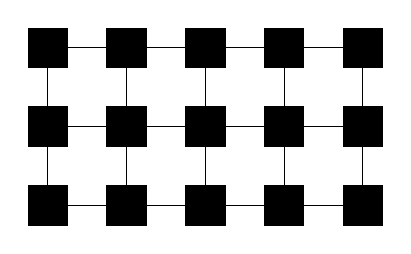
\begin{tikzpicture}
    % Set the size of each node
    \newcommand{\nodesize}{0.5cm}
  
    % Draw the grid graph
    \foreach \x in {0,1,2,3,4}
      \foreach \y in {0,1,2}
        \node [draw,fill,minimum size=\nodesize] at (\x,\y) {};
  
    % Connect the nodes horizontally
    \foreach \x in {0,1,2,3,4}
      \foreach \y [count=\nexty from 1] in {0,1}
        \draw (\x,\y) -- (\x,\nexty);
  
    % Connect the nodes vertically
    \foreach \x [count=\nextx from 1] in {0,1,2,3}
      \foreach \y in {0,1,2}
        \draw (\x,\y) -- (\nextx,\y);     
  \end{tikzpicture}
  \caption{Graf $G$} \label{fig:G1}
\end{figure}

\subsection{Złożoność problemu \textit{k}-CARD TREE}

Pokażemy, że problem drzewa Steinera, który jest powszechnie znanym z bycia silnie NP-trudnym \cite{steiner}, może być zredukowany do $k$-CARD TREE. W uprzednim problemie zadany jest podzbiór $S \subseteq V$ i próbujemy znaleźć drzewo Steinera o minimalnej wadze, czyli drzewo $T$ w $G$ takie, że $S \subseteq V(T)$ oraz $w(T)$ jest najmniejsza. Dowód redukcji znajduje się w pracy \cite{k_card_trees}.

\subsection{Najnowsze metody poszukiwania rozwiązań}

\subsubsection{Przeszukiwanie sąsiedztwa}

W pracy \cite{neighbourhood} podano wariant metody \textit{Variable neighbourhood search} (VNS \cite{vns}) przygotowany do problemu $k$-CARD TREE. Przestrzeń rozwiązań $\mathcal{S}_k$, będąca zbiorem wszystkich podrzew $T$ grafu $G$ o dokładnie $k$ krawędziach. Moc tej przestrzeni to $|\mathcal{S}_k| = \binom{n}{k+1} \cdot O(k^k)$. Odległość między dwoma drzewami $T_1$ oraz $T_2$ zdefiniowano jako:
\begin{itemize}
  \item $\rho(T_1,T_2) = |E_{T_1} \backslash E_{T_2}| = |E_{T_2} \backslash E_{T_1}|$
  \item $\eta(T_1,T_2) = |V_{T_1} \backslash V_{T_2}| = |V_{T_2} \backslash V_{T_1}|$
\end{itemize}

Wprowadzona przez Uroševića, Brimberga i Mladenovića metoda \textit{Variable neighbourhood decomposition search} (VDNS \cite{vnds}) rozszerza VNS na dwupoziomowy VNS po dekompozycji problemu.

Powyższa metoda porównana została ze standardowym VNS oraz dwoma implementacjami tabu search (TS-1 \cite{ts1}, TS-2 \cite{ts2}). Testy przeprowadzone zostały dla $n=|V|$ z przedziału [500,5000]. Na podstawie eksperymentów wykazano lepsze od konkurencji wyniki algorytmu VNDS, zarówno w postaci rozwiązań bliżej optimum, jak i krótszego czasu wykonania.

\subsubsection{Branch-and-bound}

W pracy \cite{branch_and_bound} rozszerząjącej podejścia \textit{branch-and-bound} i \textit{branch-and-cut} odpowiednio z prac \cite{integer} oraz \cite{fast} rozważany jest ukorzeniona wersja problemu $k$-CARD TREE, zwana dalej RKCTP, gdzie zadany jest wierzchołek $r \in V$, a rozwiązanie musi zawierać $r$. 

Celem zapronowanej w pracy metody jest rozwiązanie $k$-CARD TREE (zwanego tu KCTP) jako sekwencji $n-k+1$ nierosnących podproblemów RKCTP. Metoda bazowana jest na następującym pomyśle: mając zadany wierzchołek $v \in V$, weźmy $G' = G - v$. KCTP w $G$ (którego rozwiązanie przedstawmy jako KCTP($G$)) zawiera wierzchołek $v$ lub nie. Jeśli KCTP($G$) zawiera $v$, to problem zredukowany jest od RKCTP zakorzenionego w $v$ (którego optymalne rozwiązanie przedstawmy jako RKCTP($G,v$)). W przeciwnym przypadku $v$ nie należy do optymalnego rozwiązania KCTP w $G$ i może być odrzycony. Ta obserwacja prowadzi do następującego wniosku:

\[KCTP(G) = min\{RKCTP(G,v), KCTP(G')\}\]

Problem KCTP został więc sprowadzony do sekwencji podproblemów RKCTP, które będą rozwiązywane metodą \textit{branch-and-bound}. Waskie ograniczenia na optymalne rozwiązanie RKCTP z pracy \cite{rooted} oraz prosta i wydajna strategia rozgałęzień są kluczowe do minimalizacji kosztów przeszukiwania.
Aby rozwiązać RKCTP metodą \textit{branch-and-bound} definiujemy podproblem $P$ na zbiorach krawędzi $(S_1, S_0)$. Zbiór $S_1$ jest złożony z krawędzi drzewa zakorzenionego w $r$, zwanych \textit{ustalonymi krawędziami}. Zbiór $S_0$ jest zbiorem \textit{zakazanych krawędzi}. $S_1$ jest rozwiązaniem $P$ jeśli ma dokładnie $k$ krawędzi i nie ma żadnych krawędzi z $S_0$. W podproblemie $P$, jeśli $S_1$ jest rozwiązaniem to $P$ jest podproblemem terminalnym w drzewie przeszukiwań. W przeciwnym przypadku, jeśli $E\backslash(S_1 \cup S_0)$ jest niepusty to wybieramy krawędź $e$ z tego zbioru taką, że $S_1 \cup \{e\}$ też jest drzewem oraz definiujemy dwa nowe podproblemy: krawędź $e$ dodajemy do zbiorów $S_1$ albo $S_0$. Poprzez te dwie operacje podczas kroku rozgałęziania tworzone są dwa nowe podproblemy RKCTP takie, że optymalne osiągalne rozwiązanie $P$ istnieje tylko w jednej z gałęzi. W tej metodzie rozważaną krawędzią $e$ jest krawędź z $E\backslash(S_1 \cup S_0)$ o minimalnej wadze. Ponadto strategią wyboru gałęzi jest \textit{depth-first-search}.

Podczas testów metodę porównano z dwoma innymi dającymi rozwiązanie KCTP lub jego ograniczenie dolne: $k$ pierwszych kroków algorytmu Kruskala \cite{kruskal} oraz ogranicznie Kataoka'i \cite{rooted}. Zaproponowana w pracy metoda działała lepiej od obydwu wymienionych, częściej zwracając rozwiązanie optymalne oraz dając lepsze ograniczenia dolne.

\section{\textit{k}-spanning tree}

\subsection{Heurystyki}



\subsection{Algorytm hybrydowy: tabu search i kolonia mrówek}



\subsection{\textit{k}-spanning tree na okręgach}



\newpage

\bibliography{bibliography}
\bibliographystyle{ieeetr}

\end{document}